\chapter{The communication potential of FET projects on quantum technologies}
As shown in chapter \ref{FET_projects_and_social_media}, FET research projects on quantum technologies make limited use of online communication channels. In particular, none of them has considered the creation of an account on Twitter, the most common social platform among FET initiatives. It is therefore interesting to assess the community which could be reached by QT projects via Twitter.

To this aim, the following analysis was performed. First, two hashtags likely to identify tweets related to QTs were chosen. These were then monitored over disparate periods of time. The same procedure was repeated for two hashtags on HPC. The comparison of the outcomes of the two monitoring procedures provided the estimate of the communication potential of FET projects on QT via Twitter.

HPC was chosen as a comparison for the following reasons: \textit{i}) HPC and QT projects share similar communication challenges, see section \ref{Online_presence_breakdown}, and \textit{ii}) in terms of online communication, it is an active class of projects within the FET community.

This chapter is structured as follows. Sections \ref{Monitoring_of_QT_hashtags} and \ref{Monitoring_of_HPC_hashtags} outline the monitoring activity launched for the QT and HPC hashtags. The comparison of the results and the estimate of the communication potential of FET QT projects are reported in section \ref{Comparison_of_the_results}. The monitoring activities were performed with the Twitter Analytics Tool Twitonomy \cite{Twitonomy}. Twitonomy was also used to generate the plots and data presented in this chapter.

\section{Monitoring of QT hashtags} \label{Monitoring_of_QT_hashtags}
The QT hashtags monitored for the analysis presented in this chapter were \#quantumcomputing and the result of the application of the AND logic operator to \#quantum and \#technology. The former was chosen for the relevance of quantum computers in current QT research, see section \ref{FET_and_quantum_technologies}. The latter was monitored as it identifies the mentions to the overall thematic area. 

Both analyses covered two periods of time. For \#quantumcomputing, the two periods went from 7th to 14th and from 20th to 25th October 2017, respectively. As for the combination \#quantum AND \#technology, the considered time intervals covered the dates between 4th and 14th and between 15th and 25th October 2017. The time periods were chosen randomly and based on the date ranges which could be handled by the Twitonomy application given the considered volumes of tweets. Different choices of the time periods would not change the order of magnitudes of the estimates presented in this chapter.  

\begin{figure}
 \centering
 \begin{subfigure}[t]{0.9\textwidth}
   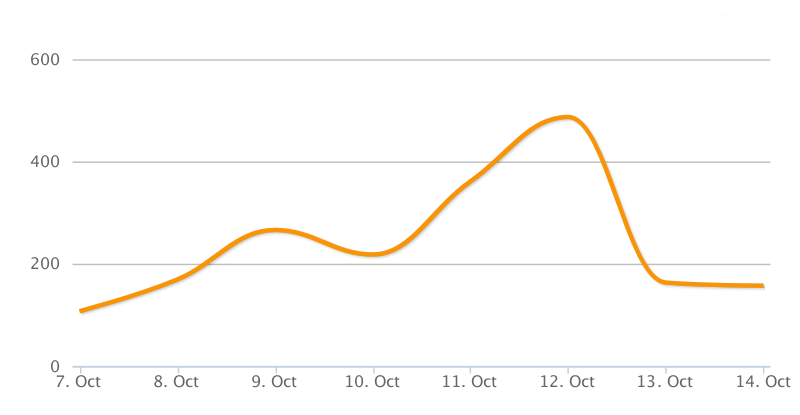
\includegraphics[width=1\linewidth]{Images/FirstSearch_QuantumComputing.png}
   \caption{} 
 \end{subfigure}

 \begin{subfigure}[t]{0.9\textwidth}
   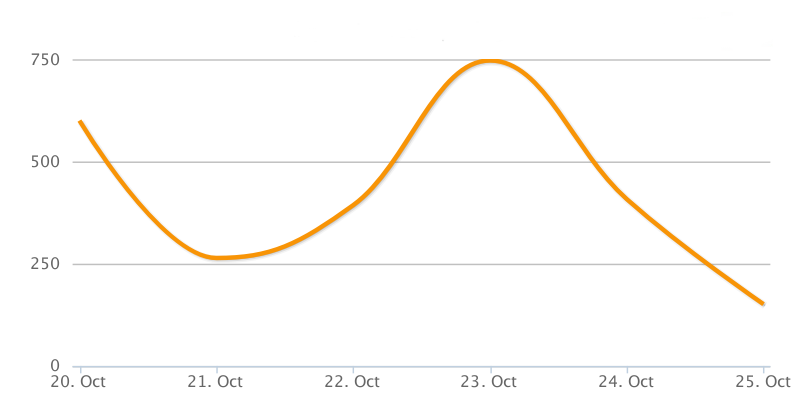
\includegraphics[width=1\linewidth]{Images/SecondSearch_QuantumComputing.png}
   \caption{}
 \end{subfigure}
 \caption{(a) Time distribution of the number of tweets with hashtag \#quantumcomputing posted between 7th and 14th October 2017. (b) As for (a) but over the time period between 20th and 25th October 2017.} 
 \label{First-SecondSearch_QuantumComputing}
\end{figure}

\begin{figure}
 \centering
 \begin{subfigure}[b]{0.9\textwidth}
   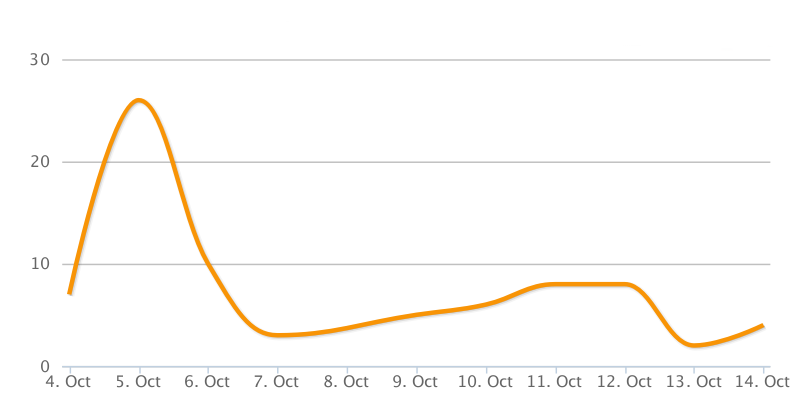
\includegraphics[width=1\linewidth]{Images/FirstSearch_QuantumTechnology.png}
   \caption{} 
 \end{subfigure}

 \begin{subfigure}[b]{0.9\textwidth}
   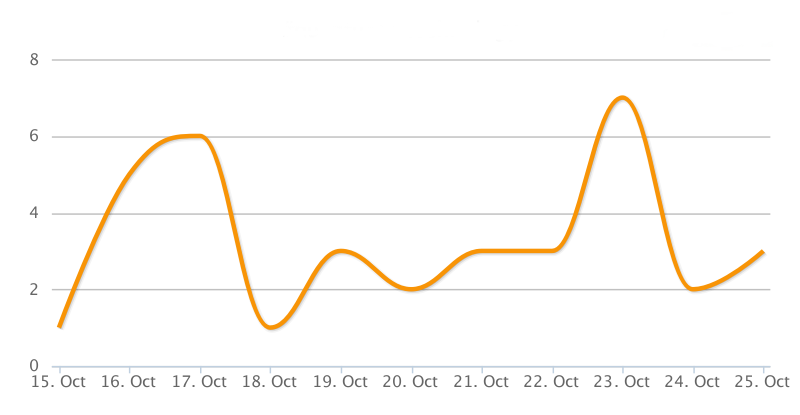
\includegraphics[width=1\linewidth]{Images/SecondSearch_QuantumTechnology.png}
   \caption{}
 \end{subfigure}
 \caption{(a) Time distribution of the number of tweets with hashtags \#quantum and \#technology posted between 4th and 14th October 2017. (b) As for (a) but over the time period between 15th and 25th October 2017.} 
 \label{First-SecondSearch_QuantumTechnology}
\end{figure}

The distribution of the number of Tweets mentioning the hashtags \#quantumcomputing and the combination \#quantum AND \#technology over the considered time periods are shown in figures \ref{First-SecondSearch_QuantumComputing} and \ref{First-SecondSearch_QuantumTechnology}, respectively. The plots indicate that, typically, the hashtag \#quantumcomputing is mentioned in hundreds of tweets each day. On the contrary, only few posts report both \#quantum and \#technology. The potential reach offered by the considered hashtags is summarised in table \ref{Summary_QuantumComputing-Technology}. The data shows that the combination \#quantum AND \#technology reaches a potential community which is significantly smaller than that of the hashtags \#quantumcomputing. 

\begin{table}[t]
 \begin{center}
 
  \begin{tabular}{cccc}
   \hline 
   \hline
   \multicolumn{4}{c}{\#quantumcomputing}\\
   \hline
   \hline
   Time period & Tweets & Users & Potential Reach \\ 
   \hline
   7 - 14 Oct 2017 & 1 928 & 1 270 & 9 392 166  \\
   20 - 25 Oct 2017 & 2 563 & 1 738 & 10 604 445  \\
   \hline
   \hline
  \end{tabular}

  \bigskip

  \begin{tabular}{cccc}
   \hline 
   \hline
   \multicolumn{4}{c}{\#quantum AND \#technology}\\
   \hline 
   \hline
   Time period & Tweets & Users & Potential Reach \\ 
   \hline
   4 - 14 Oct 2017 & 79 & 75 & 280 849  \\
   15 - 25 Oct 2017 & 36 & 28 & 85 123  \\
   \hline
   \hline
  \end{tabular}
 \end{center} 
 \caption{Summary of the Twitter analytics calculated for the hashtag \#quantumcomputing and for the combination \#quantum AND \#technology over the monitored time periods. The potential reach is defined as the total aggregate number of followers of the people who mentioned the considered keyword in their tweets.}
\label{Summary_QuantumComputing-Technology} 
\end{table}    

\section{Monitoring of HPC hashtags} \label{Monitoring_of_HPC_hashtags}
An analysis similar to the one outlined in section \ref{Monitoring_of_QT_hashtags} was conducted for the case of HPC hashtags. The considered keywords were \#HPC and \#exascale. The former is mentioned in a very large fraction of tweets on the considered topic. The latter identifies one of the key challenges embraced by the HPC community, see section \ref{FET_and_high-performing_computing}.    

For both hashtags, the considered time periods covered the dates from 4th to 14th and from 15th to 25th October 2017, respectively. The time distributions of tweets mentioning the considered keywords are shown in figures \ref{First-SecondSearch_HPC} and \ref{First-SecondSearch_Exascale}, respectively. It is worth noting that \#HPC is mentioned in hundreds of tweets per day, whereas \#exascale in, typically, few tens of tweets. 

An overview of the potential reach achievable with \#HPC and \#exascale is given in Table \ref{Summary_HPC-Exascale}. The potential reach of the \#exascale hashtag is typically one order of magnitude smaller than that of \#HPC.

\begin{table}[t]
 \begin{center}
 
  \begin{tabular}{cccc}
   \hline 
   \hline
   \multicolumn{4}{c}{\#HPC}\\
   \hline
   \hline
   Time period & Tweets & Users & Potential Reach \\ 
   \hline
   4 - 14 Oct 2017 & 2 857 & 1 372 & 11 533 160  \\
   20 - 25 Oct 2017 & 3 015 & 1 475 & 13 315 746  \\
   \hline
   \hline
  \end{tabular}

  \bigskip

  \begin{tabular}{cccc}
   \hline 
   \hline
   \multicolumn{4}{c}{\#exascale}\\
   \hline 
   \hline
   Time period & Tweets & Users & Potential Reach \\ 
   \hline
   4 - 14 Oct 2017 & 202 & 129 & 747 846 \\
   15 - 25 Oct 2017 & 207 & 164 & 1 386 972  \\
   \hline
   \hline
  \end{tabular}
 \end{center} 
 \caption{Summary of the Twitter analytics calculated for the hashtags \#HPC and \#exascale over the monitored time periods. The potential reach is defined as the total aggregate number of followers of the people who mentioned the considered keyword in their tweets.}
\label{Summary_HPC-Exascale} 
\end{table}    

\begin{figure}
 \centering
 \begin{subfigure}[b]{0.9\textwidth}
   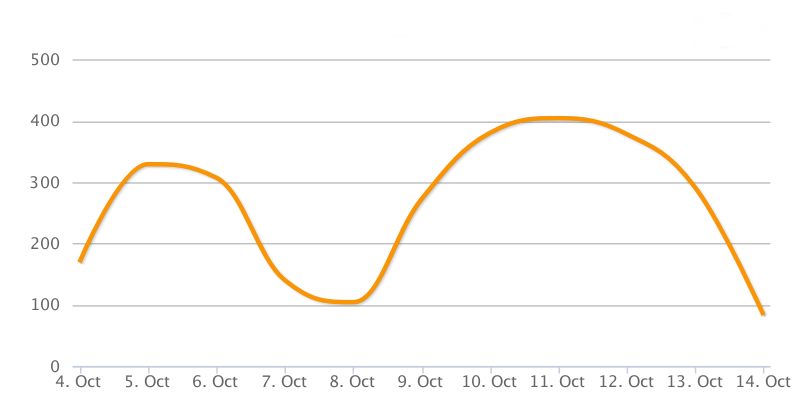
\includegraphics[width=1\linewidth]{Images/FirstSearch_HPC.png}
   \caption{} 
 \end{subfigure}

 \begin{subfigure}[b]{0.9\textwidth}
   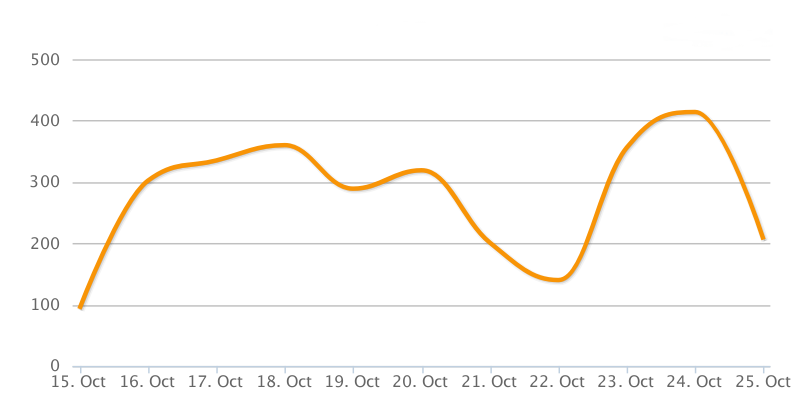
\includegraphics[width=1\linewidth]{Images/SecondSearch_HPC.png}
   \caption{}
 \end{subfigure}
 \caption{(a) Time distribution of the number of tweets with hashtag \#HPC posted between 4th and 14th October 2017. (b) As for (a) but over the time period between 15th and 25th October 2017.} 
 \label{First-SecondSearch_HPC}
\end{figure}

\begin{figure}
 \centering
 \begin{subfigure}[b]{0.9\textwidth}
   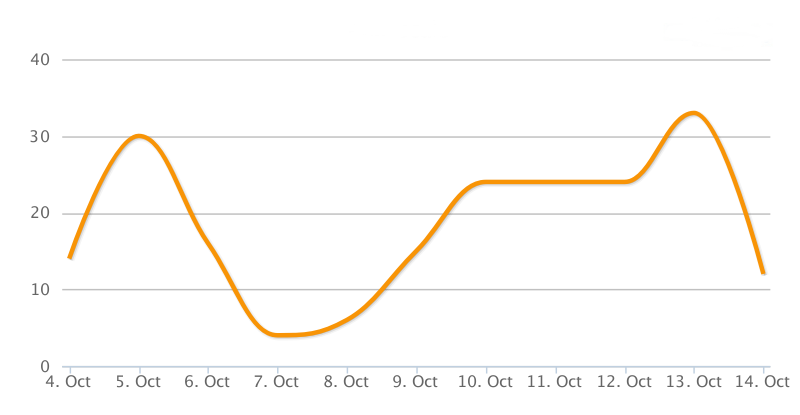
\includegraphics[width=1\linewidth]{Images/FirstSearch_Exascale.png}
   \caption{} 
 \end{subfigure}

 \begin{subfigure}[b]{0.9\textwidth}
   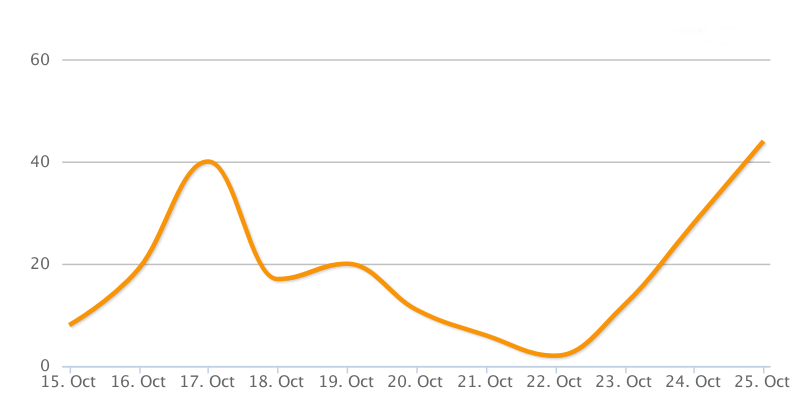
\includegraphics[width=1\linewidth]{Images/SecondSearch_Exascale.png}
   \caption{}
 \end{subfigure}
 \caption{(a) Time distribution of the number of tweets with hashtag \#exascale posted between 4th and 14th October 2017. (b) As for (a) but over the time period between 15th and 25th October 2017.} 
 \label{First-SecondSearch_Exascale}
\end{figure}

\section{Comparison of the results} \label{Comparison_of_the_results}
The monitoring activities outlined in sections \ref{Monitoring_of_QT_hashtags} and \ref{Monitoring_of_HPC_hashtags} suggest the following conclusions:

\begin{itemize}
 \item Tweets on QTs have potential reach of millions of people via Twitter. Thus, it may be worth for FET QT projects to consider Twitter as a suitable channels for communication and dissemination of research results.
 \item The potential reaches of tweets mentioning \#quantumcomputing and \#HPC share the same order of magnitude. The same holds for the total amount of tweets and users. Hence, QT projects may achieve results similar to those reported in chapter ... . 
\end{itemize}

It is interesting to note that the communities reachable by the \#quantumcomputing and \#HPC keywords are complementary. This is suggested by the plots in figure \ref{First-SecondSearch_HPC-QuantumComputing}. The plots show the time variation of the number of tweets mentioning both \#quantumcomputing and \#HPC. The amount of posts is one order of magnitude smaller than the values in figures \ref{First-SecondSearch_HPC} and \ref{First-SecondSearch_QuantumComputing}. The result is probably due to the fact that QTs and HPC pursue different strategies to improve current computers, see section \ref{Online_presence_breakdown}. As a consequence, QT projects may significantly increase the number of Twitter profiles reached by FET-funded research.

\section{Chapter summary} 
In this chapter, the following items have been discussed: 

\begin{figure}
 \centering
 \begin{subfigure}[b]{0.9\textwidth}
   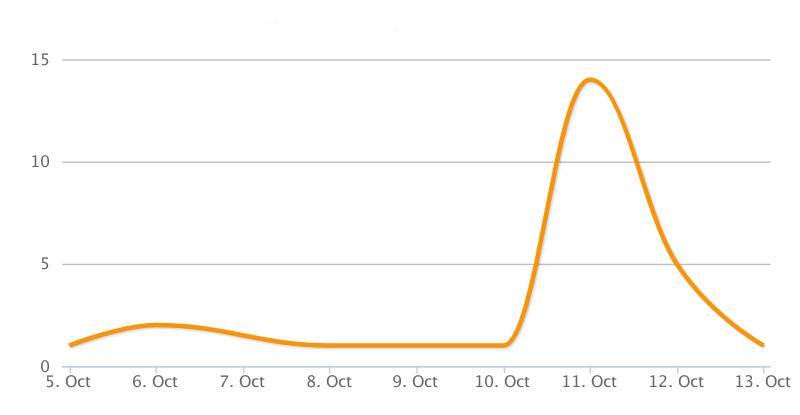
\includegraphics[width=1\linewidth]{Images/FirstSearch_HPC-QuantumComputing.png}
   \caption{} 
 \end{subfigure}

 \begin{subfigure}[b]{0.9\textwidth}
   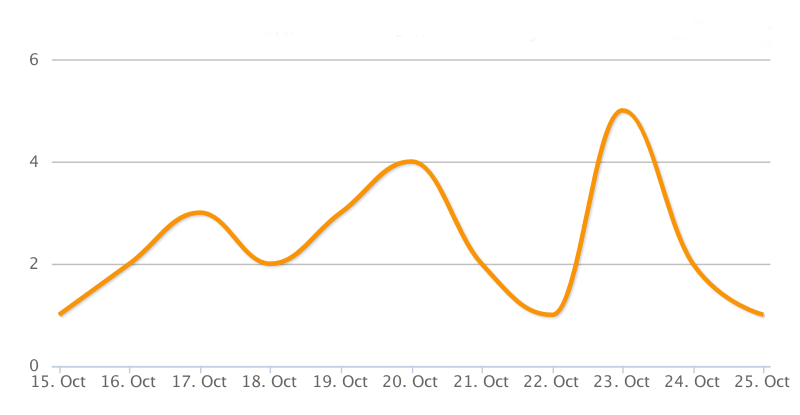
\includegraphics[width=1\linewidth]{Images/SecondSearch_HPC-QuantumComputing.png}
   \caption{}
 \end{subfigure}
 \caption{(a) Time distribution of the number of tweets with hashtags \#HPC and \#quantumcomputing posted between 5th and 13th October 2017. (b) As for (a) but over the time period between 15th and 25th October 2017.} 
 \label{First-SecondSearch_HPC-QuantumComputing}
\end{figure}